\documentclass[12pt]{beamer}
\usepackage{../Estilos/BeamerFC}
\usepackage{../Estilos/ColoresLatex}
\input{../Preambulos/pre_codigo}
\usepackage[siunitx]{circuitikz}
\usetikzlibrary{arrows,patterns,shapes}
\usetikzlibrary{decorations.markings}
\usetikzlibrary{arrows}
\input{../Preambulos/preambulo_Beamer_Copenhagen_wolverine}
\usefonttheme{serif}

\title{\large{Métodos adaptativos}}
\subtitle{Tema 3 - Ecuaciones Diferenciales Ordinarias}
\author{M. en C. Gustavo Contreras Mayén}
\date{}

\begin{document}
\maketitle

\section{Método Predictor-Corrector Euler}
\frame{\tableofcontents[currentsection, hideothersubsections]}
\subsection{Ejercicio 2}

\begin{frame}
\frametitle{Enunciado del ejercicio}
El récord mundial de lanzamiento de martillo masculino es de $\SI{86.74}{\meter}$ y pertenece a Yuriy Sedykh desde 1986.
\\
\bigskip
\pause
El martillo masculino pesa $\SI{7.26}{\kilo\gram}$, es esférico y tiene un radio típico $R = \SI{6}{\centi\meter}$.
\end{frame}
\begin{frame}
\frametitle{Enunciado del ejercicio}
El arrastre del martillo se puede considerar proporcional al cuadrado de la velocidad del martillo en relación con el aire:
\pause
\begin{align*}
F_{\text{D}} = \dfrac{1}{2} \, \rho \, A \, C_{\text{D}} \, v^{2}
\end{align*}
\pause
Donde:
\setbeamercolor{item projected}{bg=aquamarine,fg=arsenic}
\setbeamertemplate{enumerate items}{%
\usebeamercolor[bg]{item projected}%
\raisebox{1.5pt}{\colorbox{bg}{\color{fg}\footnotesize\insertenumlabel}}%
}
\begin{enumerate}[<+->]
\item $\rho$ es la densidad del aire $= \SI{1.2}{\kilo\gram\per\cubic\meter}$
\item $A = \pi \, R^{2}$ es la sección de área del martillo.
\end{enumerate}
\end{frame}
\begin{frame}
\frametitle{Tipos de flujo}
El martillo puede experimentar, en principio, un flujo \enquote{\textcolor{cerise}{laminar separado}}, con un coeficiente de arrastre típico $C_{d} = 0.5$, \pause o un flujo \enquote{\textcolor{cobalt}{inestable-oscilante}}, con $C_{d} = 0.75$.
\end{frame}
\begin{frame}
\frametitle{Incisos a resolver}
Considera los lanzamientos desde la posición inicial $x_{0} = 0$, $y_{0} = \SI{2}{m}$, bajo el ángulo ideal $\varphi = \ang{45}$:
\pause
\setbeamercolor{item projected}{bg=cornellred,fg=cosmiclatte}
\setbeamertemplate{enumerate items}{%
\usebeamercolor[bg]{item projected}%
\raisebox{1.5pt}{\colorbox{bg}{\color{fg}\footnotesize\insertenumlabel}}%
}
\begin{enumerate}[<+->]
\item Encuentra la velocidad inicial que produce la distancia de lanzamiento del récord mundial.
\seti
\end{enumerate}
\end{frame}
\begin{frame}
\frametitle{Incisos a resolver}
\setbeamercolor{item projected}{bg=cornellred,fg=cosmiclatte}
\setbeamertemplate{enumerate items}{%
\usebeamercolor[bg]{item projected}%
\raisebox{1.5pt}{\colorbox{bg}{\color{fg}\footnotesize\insertenumlabel}}%
}
\begin{enumerate}[<+->]
\conti
\item Resuelve la ecuación de movimiento de Newton para el lanzamiento oblicuo del martillo usando el método predictor-corrector de Euler con un paso de tiempo $h = 0.01$, transformando primero las EDO para los movimientos $x$ e $y$ en un sistema de cuatro EDO1.
\seti
\end{enumerate}
\end{frame}
\begin{frame}
\frametitle{Incisos a resolver}
\setbeamercolor{item projected}{bg=cornellred,fg=cosmiclatte}
\setbeamertemplate{enumerate items}{%
\usebeamercolor[bg]{item projected}%
\raisebox{1.5pt}{\colorbox{bg}{\color{fg}\footnotesize\insertenumlabel}}%
}
\begin{enumerate}[<+->]
\conti
\item Calcula y grafica la dependencia temporal de la altitud del martillo y su trayectoria $y = y (x)$ en tres regímenes de flujo:
\\
a) Sin fricción. \\
b) Flujo laminar separado. \\
c) Flujo oscilante inestable.
\item Evalúa la cantidad por la cual la distancia de tiro está influenciada por el arrastre.
\end{enumerate}
\end{frame}
\begin{frame}
\frametitle{Inciso 1}
\textbf{Ejercicio a cuenta:} Plantea el problema a partir de la información que nos da el enunciado y resuelve el correspondiente sistema, para demostrar que la velocidad inicial con la que se alcanza la distancia del lanzamiento que es récord mundial es:
\pause
\begin{align*}
v_{0} =  \SI{25}{\meter\per\second}
\end{align*}
\end{frame}
\begin{frame}
\frametitle{Inciso 2}
El problema equivalente con el conjunto de EDO1 es el siguiente: \pause con la notación:
\pause
\begin{align*}
y_{1} &= x \\
y_{2} &= y \\
y_{3} &= v_{x} \\
y_{4} &= v_{y} \\
\end{align*}
\end{frame}
\begin{frame}
\frametitle{En modo de arreglos}
Se tiene entonces que:
\pause
\begin{align*}
\begin{bmatrix}
\pderivada{y}_{1} \\
\pderivada{y}_{2} \\
\pderivada{y}_{3} \\
\pderivada{y}_{4} 
\end{bmatrix}
= 
\begin{bmatrix}
y_{3} \\
y_{4} \\
- \bigg( \dfrac{k}{m} \bigg) \, y_{3} \abs{y_{3}} \\
- \bigg( \dfrac{k}{m} \bigg) \, y_{4} \abs{y_{4}}
\end{bmatrix}
\hspace{1.5cm}
\begin{bmatrix}
y_{1} (0) \\
y_{2} (0) \\
y_{3} (0) \\
y_{4} (0)
\end{bmatrix}
=
\begin{bmatrix}
x_{0} \\
y_{0} \\
v_{x0} \\
v_{y0}
\end{bmatrix}
\end{align*}
\end{frame}
\begin{frame}
\frametitle{Resolviendo para $C_{D} = 0.5$}
Se presenta la solución al ejercicio con el flujo \enquote{\textcolor{cerise}{laminar separado}}: $C_{D} = 0.5$.
\\
\bigskip
\pause
\textbf{Ejercicios a cuenta (2)}: Obtener las soluciones, las gráficas para los casos: sin fricción y con el flujo \enquote{\textcolor{cobalt}{inestable-oscilante}}, con $C_{d} = 0.75$. Así como una gráficas con las tres soluciones simultáneas.
\end{frame}
\begin{frame}[allowframebreaks, fragile]
\frametitle{Código para la solución}
El siguiente código presenta la parte central de la solución, para evitar varias diapositivas con las constantes, te pedimos que revises el notebook para que se complemente el código.
\end{frame}
\begin{frame}[allowframebreaks, fragile]
\frametitle{Código para la solución}
\begin{lstlisting}[caption=Código con el método Corrector-Predictor de Euler]
from metodosDirectos import eulerPC
import numpy as np

def Func(t, y, f):
    f[1] = y[3]
    f[2] = y[4]
    f[3] = -k/m * y[3]*np.fabs(y[3])
    f[4] = -k/m * y[4]*np.fabs(y[4]) - g

y[1] = x0 ; y[2] = y0
y[3] = vx0; y[4] = vy0

tt[1] = t
xt[1] = y[1]; yt[1] = y[2]

while (t + ht <= tmax):
    eulerPC(t, ht, y, n, Func)
    t += ht; it += 1
   
    tt[it] = t
    xt[it] = y[1]; yt[it] = y[2]
   
    if (y[2] < 0.e0): break
\end{lstlisting}
\end{frame}
\begin{frame}
\frametitle{De las gráficas}
El código en el notebook no incluye los procedimientos para determinar:
\setbeamercolor{item projected}{bg=bananayellow,fg=black}
\setbeamertemplate{enumerate items}{%
\usebeamercolor[bg]{item projected}%
\raisebox{1.5pt}{\colorbox{bg}{\color{fg}\footnotesize\insertenumlabel}}%
}
\begin{enumerate}[<+->]
\item La altura máxima.
\item La distancia que recorre el martillo.
\item La rutina de graficación.
\end{enumerate}
\pause
Por lo que deberás de aplicar lo que hemos aprendido tanto de la física como de \python, para responder debidamente. La siguiente gráfica es un ejemplo de la respuesta esperada.
\end{frame}
\begin{frame}
\frametitle{Gráfica de la altura máxima}
\begin{figure}
    \centering
    \includegraphics[scale=0.55]{Imagenes/plot_eulerPC_ejercicio_02_02.eps}
\end{figure}
\end{frame}
\begin{frame}
\frametitle{Gráfica de la distancia máxima}
\begin{figure}
    \centering
    \includegraphics[scale=0.55]{Imagenes/plot_eulerPC_ejercicio_02_01.eps}
\end{figure}
\end{frame}



% \begin{frame}
% \frametitle{Ejemplo}
% Mostrar que el problema
% \[ y'' = - \dfrac{19}{4}y - 10 y', \hspace{1cm} y(0)=-9, \hspace{1cm} y'(0)=0 \]
% \begin{enumerate}
% \item Es ''moderadamente'' rígido.
% \item Estimar el valor de $h_{max}$, el valor mayor de $h$ con el cual el método RK es estable. \item Revisa al calcular $y(10)$ con $h \simeq h_{max}/2$ y $h \simeq 2 h_{max}$.
% \end{enumerate}
% \end{frame}
% \begin{frame}
% \frametitle{Solución Punto 1}
% Con la notación que ya manejamos, hacemos $y=y_{0}$ y $y'=y_{1}$, para nuestro sistema de EDO-1
% \[ \mathbf{y}' = \begin{bmatrix}
% y_{1} \\
% - \dfrac{19}{4} y_{0} - 10 y_{1}
% \end{bmatrix}  =
% - \mathbf{\Lambda}
% \begin{bmatrix}
% y_{0} \\
% y_{1}
% \end{bmatrix}
% \]
% \pause
% donde
% \[ \mathbf{\Lambda} = 
% \begin{bmatrix}
% 0 & -1 \\
% \dfrac{19}{4} & 10
% \end{bmatrix}
% \]
% \end{frame}
% \begin{frame}
% Los valores propios de $\mathbf{\Lambda}$ están dados por
% \[ \vert \mathbf{\Lambda} - \lambda \mathbf{I} \vert = 
% \begin{vmatrix}
% - \lambda & -1 \\
% \dfrac{19}{4} & 10 - \lambda
% \end{vmatrix} = 0 \]
% Que nos devuelve $\lambda_{1} = 1/2$ y $\lambda_{2} = 19/2$.
% \\
% \medskip
% Como $\lambda_{2}$ es un poco más grande que $\lambda_{1}$, las ecuaciones son ''moderadamente'' rígidas.
% \end{frame}
% \begin{frame}
% \frametitle{Solución Punto 2}
% Un estimado para el límite superior de $h$ en donde es estable el método se puede obtener de la expresión indicada anteriormente
% \[ h_{max} = \dfrac{2}{\lambda_{max}} = \dfrac{2}{19/2} = 0.2153\]
% Aunque esta fórmula es válida estrictamente para el método de Euler, por lo general se puede utilizar para las fórmulas de integración de orden superior.
% \end{frame}
% \begin{frame}
% \frametitle{Solución Punto 3}
% Haciendo $h_{1} = \lambda_{max}/2 = 0.10765 \simeq 0.1$ y ejecutando el código, tenemos que
% \begin{tabular}{c | c | c}
% $x$ & $y[0]$ & $y[1]$ \\ \hline
% $0.0000e+000$ & $-9.0000e+000$ & $0.0000e+000$ \\ \hline
% $1.0000e+001$ & $-6.4011e-002$ & $3.2005e-002$ \\ \hline
% \end{tabular}
% \\
% \medskip
% La solución analítica del problema es:
% \[ y(x) = -\dfrac{19}{2} \exp \left( - \frac{x}{2} \right) + \dfrac{1}{2} \exp \left(- \frac{19x}{2} \right) \]
% evaluando $y(10)= 0.064011$, que es el valor que se obtiene con el método RK4.
% \end{frame}
% \begin{frame}
% Ahora haciendo $h_{2} = 2 \lambda_{max} = 0.4306$ y ejecutando nuevamente el código, tenemos que
% \begin{tabular}{c | c | c}
% $x$ & $y[0]$ & $y[1]$ \\ \hline
% $0.0000e+00$ & $-9.0000e+00$ & $0.0000e+00$ \\ \hline
% $1.0000e+01$ & $1.9244e+16$ & $-1.8282e+17$ \\ \hline
% \end{tabular}
% \\
% \medskip
% En donde vemos que la inestabilidad del método se hace evidente por el valor de $h$.
% \end{frame}

\section{Métodos multipaso}
\frame{\tableofcontents[currentsection, hideothersubsections]}
\subsection{Definición}

\begin{frame}
\frametitle{Métodos multipaso}
La determinación del tamaño de $h$ adecuado, puede ser un dolor de cabeza en los procedimientos de integración numérica:
\pause
\setbeamercolor{item projected}{bg=americanrose,fg=antiquewhite}
\setbeamertemplate{enumerate items}{%
\usebeamercolor[bg]{item projected}%
\raisebox{1.5pt}{\colorbox{bg}{\color{fg}\footnotesize\insertenumlabel}}%
}
\begin{enumerate}[<+->]
\item Si es demasiado grande, el error de truncamiento resulta ser inaceptable.
\item Si su demasiado pequeño, estamos desperdiciando recursos computacionales.
\end{enumerate}
\end{frame}
\begin{frame}
\frametitle{Métodos multipaso}
Por otra parte, un tamaño de paso constante puede no ser adecuado para toda la gama de integración.
\\
\bigskip
\pause
Por ejemplo, si la curva solución comienza con cambios rápidos antes de convertirse en suave (como en un problema de rigidez), debemos utilizar una $h$ pequeña al principio y aumentarla cuando llegamos a la zona lisa.
\end{frame}
\begin{frame}
\frametitle{Métodos adaptativos}
Aquí es donde los \textbf{\textcolor{carmine}{métodos adaptativos}} llegan para apoyarnos: \pause estiman el error de truncamiento en cada paso de integración y ajustan automáticamente el tamaño de paso para mantener el error dentro de los límites prescritos.
\end{frame}
\begin{frame}
\frametitle{Fórmulas de integración}
Los métodos de Runge-Kutta adaptativos utilizan las denominadas \textbf{\textcolor{blue}{fórmulas de integración incorporadas}}.
\\
\medskip
\pause
Estas fórmulas vienen en pares: \pause una fórmula tiene el orden de integración $m$, \pause la otra es de orden $m + 1$.
\\
\bigskip
\pause
 La idea es utilizar ambas fórmulas para avanzar en la solución de $x$ a $x + h$.
\end{frame}
\begin{frame}
\frametitle{Fórmulas de integración}
De los resultados $\mathbf{y}_{m}(x+h)$ e $\mathbf{y}_{m+1}(x+h)$ podemos estimar el error de truncamiento en la fórmula de orden $m$:
\pause
\begin{align*}
\mathbf{E}(h) = \mathbf{y}_{m+1} (x + h) - \mathbf{y}_{m} (x + h)
\end{align*}
Lo que hace atractivo el uso de fórmulas embebidas, ya que comparten puntos donde $\mathbf{F} (x, \mathbf{y})$ son evaluados.
\end{frame}
\begin{frame}
\frametitle{Requerimiento adicional}
Esto significa que cada $\mathbf{y}_{m} (x + h)$ ha sido calculado, entonces se requiere un esfuerzo pequeño para calcular $\mathbf{y}_{m+1} (x + h)$
\end{frame}

\subsection{Fórmulas Runge-Kutta-Fehlberg}

\begin{frame}
\frametitle{Fórmulas Runge-Kutta-Fehlberg}
Se presentan las fórmulas incoporadas de orden 5 y 4 obtenidas por Erwin Fehlberg, por lo que se conocen como las fórmulas Runge-Kutta-Felhlberg (RKF45):
\pause
\begin{align*}
\mathbf{K}_{0} &= h \, \mathbf{F} (x, y) \\
\mathbf{K}_{i} &= h \, \mathbf{F} \left( x + A_{i} \, h, \mathbf{y} + \nsum_{j=0}^{i-1} B_{ij} \, \mathbf{K}_{j} \right) \\
{}& \hspace{3cm} i = 1, 2, \ldots, 6
\end{align*}
\end{frame}
\begin{frame}
\frametitle{Fórmulas Runge-Kutta-Fehlberg}
La fórmula de quinto orden es:
\pause
\begin{align*}
\mathbf{y}_{5} (x + h) = \mathbf{y} (x) + \nsum_{i=0}^{6} C_{i} \, \mathbf{K}_{i}
\end{align*}
\pause
Mientras que la fórmula de cuarto orden es:
\begin{align*}
\mathbf{y}_{4} (x + h) = \mathbf{y} (x) + \nsum_{i=0}^{6} D_{i} \, \mathbf{K}_{i}
\end{align*}
\end{frame}
\begin{frame}
\frametitle{Coeficientes necesarios}
Los coeficientes que aparecen en las fórmulas no son únicos.
\\
\bigskip
\pause
En la siguiente tabla se muestran los valores de los coeficientes. \pause Se afirma que proporcionan una predicción de errores superior a los valores alternativos.
\end{frame}
\begin{frame}
\frametitle{Tabla de coeficientes}
\begin{table}
\centering
\renewcommand*{\arraystretch}{0.9}
\begin{tabular}{| c | c | c c c c c  c | c | c |}
\hline
$i$ & $A_{i}$ & & & $B_{ij}$ & & & & $C_{i}$ & $D_{i}$ \\ \hline
$\scriptstyle 0$ & - & - & - & - & - & - & & $\frac{35}{384}$ & $\frac{5179}{57600}$ \\ \hline
$\scriptstyle 1$ & $\frac{1}{5}$ & $\frac{1}{5}$ & - & - & - & - & & $\scriptstyle 0$ & $\scriptstyle 0$ \\ \hline
$\scriptstyle 2$ & $\frac{3}{10}$ & $\frac{3}{40}$ & $\frac{9}{40}$ & - & - & - & & $\frac{250}{621}$ & $\frac{18575}{48384}$ \\ \hline
$\scriptstyle 3$ & $\frac{4}{5}$ & $\frac{44}{45}$ & $-\frac{56}{15}$ & $\frac{32}{9}$ & - & - & & $\frac{125}{192}$ & $\frac{393}{640}$ \\ \hline
$\scriptstyle 4$ & $\frac{8}{9}$ & $\frac{19372}{6561}$ & $-\frac{25360}{2187}$ & $\frac{64448}{6561}$ & $-\frac{212}{729}$ & - &  &$\frac{-2187}{6784}$ & $\frac{92097}{339200}$ \\ \hline
$\scriptstyle 5$ & $\scriptstyle 1$ & $\frac{9017}{3168}$ & $-\frac{355}{5}$ & $\frac{46732}{5247}$ & $\frac{49}{176}$ & $-\frac{5103}{18656}$ & & $\frac{11}{84}$ & $\frac{187}{2100}$ \\ \hline
$\scriptstyle 6$ & $\scriptstyle 1$ & $\frac{35}{384}$ & $\scriptstyle 0$ & $\frac{500}{1113}$ & $\frac{125}{192}$ & $-\frac{2187}{6784}$ &  $\frac{11}{84}$ & $\scriptstyle 0$ & $\frac{1}{40}$ \\ \hline
\end{tabular}
\end{table}
\end{frame}

\subsection{Sobre el error}

\begin{frame}
\frametitle{Estimación del error}
La solución de un problema se avanza con la fórmula de quinto orden en la ecuación.
\\
\bigskip
\pause
La fórmula de cuarto orden se usa solo implícitamente al estimar el error de truncamiento.
\pause
\begin{align*}
\mathbf{E} (h) = \mathbf{y}_{5} (x + h) - \mathbf{y}_{5} (x + h) = \nsum_{i=0}^{6} \big( C_{i} - D_{i} \big) \, \mathbf{K}_{i}
\end{align*}
\end{frame}
\begin{frame}
\frametitle{Estimación del error}
La ecuación anterior en realidad se aplica a la fórmula de cuarto orden, \pause tiende a sobrestimar el error en la fórmula de quinto orden.
\end{frame}
\begin{frame}
\frametitle{Estimación del error}
Tengamos en cuenta que $\mathbf{E} (h)$ es un vector, sus componentes $E_{i} (h)$ representan los errores en las variables dependientes $y_{i}$.
\\
\bigskip
\pause
Esto plantea la pregunta:
\\
\pause
\textbf{¿Cuál es la medida de error $e (h)$ que deseamos controlar?}
\end{frame}
\begin{frame}
\frametitle{Estimación del error}
No existe una sola opción que funcione bien en todos los problemas.
\\
\bigskip
\pause
Si queremos controlar el componente más grande de $\mathbf{E} (h)$, la medida del error sería:
\pause
\begin{align*}
e (h) = \max_{i} \abs{E_{i} (h)}
\end{align*}
\end{frame}
\begin{frame}
\frametitle{Estimación del error}
También podríamos controlar alguna medida bruta del error, como el error cuadrático medio definido por:
\pause
\begin{align*}
\tilde{\mathbf{E}} (h) = \sqrt{\dfrac{1}{n} \, \nsum_{i=0}^{n-1} E_{i}^{2} (h)}
\end{align*}
donde $n$ es el número de ecuaciones de quinto orden.
\end{frame}
\begin{frame}
\frametitle{Estimación del error}
Entonces usaríamos:
\pause
\begin{align*}
e (h) = \tilde{E} (h)
\end{align*}
para la medida del error.
\\
\bigskip
\pause
Dado que el error de raíz cuadrática media es más fácil de manejar, lo adoptamos para nuestro código.
\end{frame}
\begin{frame}
\frametitle{Tolerancia para el error}
El control del error se logra ajustando el incremento $h$ de modo que el error por paso $e (h)$ sea aproximadamente igual a una tolerancia prescrita $\varepsilon$.
\end{frame}
\begin{frame}
\frametitle{Error por truncamiento}
Observando que el error de truncamiento en la fórmula de cuarto orden es $\order{h^{5}}$, concluimos que:
\pause
\begin{align*}
\dfrac{e (h_{1})}{e (h_{2})} \approx \bigg( \dfrac{h_{1}}{h_{2}} \bigg)^{5}
\end{align*}
\end{frame}
\begin{frame}
\frametitle{Ajuste en el paso de integración}
Supongamos que realizamos un paso de integración con $h_{1}$ que resultó en el error $e (h_{1})$.
\\
\bigskip
\pause
El tamaño de paso $h_{2}$ que deberíamos haber usado ahora se puede obtener de la ecuación anterior, haciendo que $e (h_{2}) = \varepsilon$:
\pause
\begin{align*}
h_{2} = h_{1} \, \bigg[ \dfrac{\varepsilon}{e (h_{1})} \bigg]^{\frac{1}{5}}
\end{align*}
\end{frame}
\begin{frame}
\frametitle{Condición para repetir la integración}
Si $h_{2} \geq h_{1}$, podríamos repetir el paso de integración con $h_{2}$, pero debido a que el error estaba por debajo de la tolerancia, sería un desperdicio de un resultado perfectamente bueno.
\\
\bigskip
\pause
Entonces aceptamos el paso actual y probamos $h_{2}$ en el siguiente paso. \pause Sin embargo, si $h_{2} < h_{1}$, debemos desechar el paso actual y repetirlo con $h_{2}$.
\end{frame}
\begin{frame}
\frametitle{Sentido de la aproximación}
Porque la ecuación anterior es solo una aproximación cruda, \pause es prudente incorporar un pequeño margen de seguridad.
\\
\bigskip
\pause
En nuestro código usaremos:
\pause
\begin{align*}
h_{2} = 0.9 \, h_{1} \, \bigg[ \dfrac{\varepsilon}{e (h_{1})} \bigg]^{\frac{1}{5}}
\end{align*}
\pause 
También evitamos cambios excesivamente grandes en $h$ aplicando las restricciones:
\pause
\begin{align*}
0.1 \leq \dfrac{h_{2}}{h_{1}} \leq 10
\end{align*}
\end{frame}
\begin{frame}
\frametitle{Error truncamiento local}
Recordemos que $e (h)$ se aplica a un solo paso de integración; es decir, es una medida del error de truncamiento local.
\\
\bigskip
\pause
El importantísimo error de truncamiento global es causado por la acumulación de errores locales.
\end{frame}
\begin{frame}
\frametitle{Pregunta relevante}
¿Cómo debe establecerse $\varepsilon$ para lograr una tolerancia de error global global?
\\
\bigskip
\pause
Debido a que $e (h)$ es una estimación conservadora del error real, \pause hacer que $\varepsilon = \varepsilon_{\text{global}}$ suele ser adecuado. \pause Si el número de pasos de integración es muy grande, es recomendable disminuir $\varepsilon$ en consecuencia.
\end{frame}
\begin{frame}
\frametitle{Otra pregunta relevante}
\textbf{\textcolor{red}{¿Hay alguna razón para usar los métodos no adaptativos?}}
\\
\bigskip
\pause
Por lo general, no; \pause sin embargo, hay casos especiales en los que los métodos adaptativos fallan.
\end{frame}
\begin{frame}
\frametitle{Casos particulares}
Por ejemplo, los métodos adaptativos generalmente no funcionan si $\mathbf{F} (x, \mathbf{y})$ contiene discontinuidades.
\\
\bigskip
\pause
Debido a que el error se comporta de manera errática en el punto de discontinuidad, el programa puede quedarse atascado en un ciclo infinito tratando de encontrar el valor apropiado de $h$. %Los métodos no adaptativos también son útiles si la salida debe tener valores de x espaciados uniformemente.
\end{frame}

\subsection{La función \texttt{run\_kut5}}

\begin{frame}
\frametitle{Preparando la función}
El argumento de entrada $h$ es el valor de prueba del incremento para el primer paso de integración.
\\
\bigskip
\pause
Tengamos en cuenta que $K_{0}$ se calcula desde cero solo en el primer paso de integración.
\end{frame}
\begin{frame}
\frametitle{Calculando $\textbf{K}_{0}$}
Posteriormente, usaremos:
\pause
\begin{align*}
\big( \mathbf{K}_{0} \big)_{m+1} = \dfrac{h_{m+1}}{h_{m}} \, \big( \mathbf{K}_{6} \big)_{m}
\end{align*}
\pause
si el m-ésimo paso se aceptó.
\end{frame}
\begin{frame}
\frametitle{Calculando $\textbf{K}_{0}$}
Y se utilizará:
\pause
\begin{align*}
\big( \mathbf{K}_{0} \big)_{m+1} = \dfrac{h_{m+1}}{h_{m}} \, \big( \mathbf{K}_{0} \big)_{m}
\end{align*}
\pause
si el m-ésimo paso se rechazó debido al excesivo error por truncamiento.
\end{frame}
\begin{frame}
\frametitle{Revisión del código}
El código \funcionazul{integra\_RKAdaptativo} se ha incluido en el módulo \funcionazul{metodosDirectos}, \pause revisarlo aquí en la presentación sería extendido, mejor veremos su uso en la solución de un ejercicio.
\end{frame}

\subsection{Ejercicios método RK-Adaptativo}

\begin{frame}
\frametitle{Enunciado del ejercicio 1}
La fuerza de arrastre aerodinámico en un objeto en caída libre se puede aproximar por la expresión:
\pause
\begin{align*}
F_{D} = a \, v^{2} \, \exp(-by)
\end{align*}
donde:
\pause
\setbeamercolor{item projected}{bg=bazaar,fg=blond}
\setbeamertemplate{enumerate items}{%
\usebeamercolor[bg]{item projected}%
\raisebox{1.5pt}{\colorbox{bg}{\color{fg}\footnotesize\insertenumlabel}}%
}
\begin{enumerate}[<+->]
\item $v$ es la velocidad del objeto en m/s.
\item $y$ es la elevación del objeto en metros.
\item $a = \SI{7.45}{\kilo\gram\per\metre}$
\item $b = \SI{10.53d-5}{\per\metre}$
\end{enumerate}
\end{frame}
\begin{frame}
\frametitle{La ED que modela el problema}
El término exponencial representa el cambio de densidad del aire con la elevación.
\\
\bigskip
\pause
La ecuación diferencial que describe la caída del objeto es:
\pause
\begin{align*}
m \, \ddot{y} = - m \, g + F_{D}
\end{align*}
donde $g = \SI{9.81}{\meter\per\square\second}$ y $ m = \SI{114}{\kilo\gram}$ es la masa del objeto.
\end{frame}
\begin{frame}
\frametitle{Problema a resolver}
Si el objeto se libera de una altura de $\SI{9}{\kilo\meter}$.
\\
\bigskip
\pause
\textbf{\textcolor{burgundy}{Calcula su altura y velocidad}} luego de $10$ segundos de caída, utiliza el método RK adaptativo.
\end{frame}
\begin{frame}
\frametitle{Planteamiento para la solución}
La ecuación diferencial y las condiciones iniciales son:
\pause
\begin{align*}
\ddot{y} &= - g + \dfrac{a}{m} \, \dot{y}^{2} \, \exp(-b \, y) \\
&= -9.81 + \dfrac{7.45}{114} \, \dot{y}^{2} \, \exp(\num{-10.53d-5} \, y) \\
{} \\
&{} y(0) = \SI{9000}{\meter} \hspace{1cm} \dot{y}(0) = 0
\end{align*}
\end{frame}
\begin{frame}
\frametitle{Usando la notación}
Haciendo $y_{0} = y$ y $y_{1} = \dot{y}$, obtenemos el sistema de EDO1:
\pause
\begin{align*}
\mathbf{\dot{y}} &= \begin{bmatrix}
\dot{y}_{0} \\
\dot{y}_{1}
\end{bmatrix} \\
&= \begin{bmatrix}
y_{1} \\
-9.80665 + (\num{65.351d-3}) \, y_{1}^{2} \, \exp(\num{-10.53d-5} y_{0})
\end{bmatrix}
\end{align*}
\end{frame}
\begin{frame}
\frametitle{Usando la notación}
\begin{align*}
\mathbf{y}(0) = 
\begin{bmatrix}
9000 \mbox{ m} \\
0
\end{bmatrix}
\end{align*}
\end{frame}
\begin{frame}
\frametitle{Código subsecuente}
Revisemos el notebook de Jupyter.
\\
\bigskip
\pause
Considera que hay que completar el código, lo que debes de mostrar en la sesión es la siguiente gráfica y los resultados solicitados de la altura del móvil y su velocidad a los $\SI{10}{\second}$ del lanzamiento.
\end{frame}
\begin{frame}
\frametitle{Gráfica que se debe elaborar}
\begin{figure}
    \centering
    \includegraphics[scale=0.55]{Imagenes/Ejercicio_RKAdaptativo_01.eps}
\end{figure}
\end{frame}
\begin{frame}
\frametitle{Ejercicio 2}
En este ejercicio se presenta de manera visual el procedimiento adaptativo al paso de integración $h$.
\\
\bigskip
\pause
El enunciado y lo que hay que resolver en el notebook de Jypyter. Nuevamente hay que graficar los resultados.
\end{frame}
\begin{frame}
\frametitle{Densidad de puntos evaluados}
\begin{figure}
    \centering
    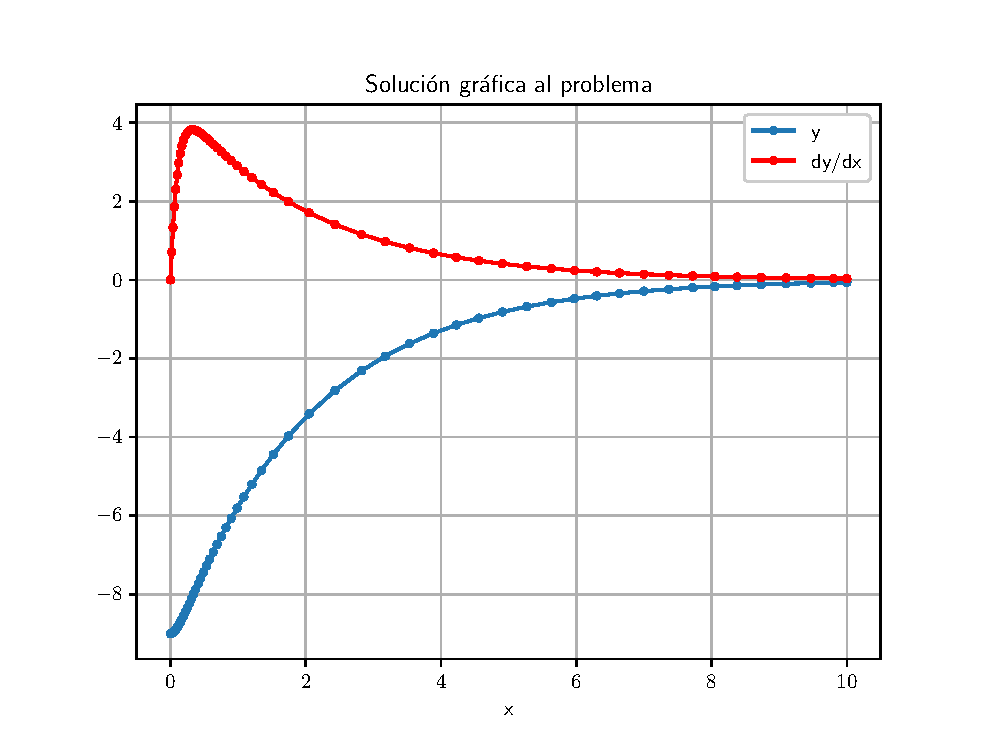
\includegraphics[scale=0.55]{Imagenes/Ejercicio_RKAdaptativo_02.eps}
\end{figure}
\end{frame}


\subsection{Ejercicios a cuenta}

\begin{frame}
\frametitle{Ejercicios a cuenta}
\setbeamercolor{item projected}{bg=blue,fg=yellow}
\setbeamertemplate{enumerate items}{%
\usebeamercolor[bg]{item projected}%
\raisebox{1.5pt}{\colorbox{bg}{\color{fg}\footnotesize\insertenumlabel}}%
}
\begin{enumerate}
\item Considera el problema:
\begin{align*}
\pderivada{y} = x - 10 \, y \hspace{1.5cm} y (0) = 10
\end{align*}
En la siguiente diapositiva se indican los enunciados que debes de responder para este problema.
\seti
\end{enumerate}
\end{frame}
\begin{frame}
\frametitle{Por resolver}
\setbeamercolor{item projected}{bg=canaryyellow,fg=cerise}
\setbeamertemplate{enumerate items}{%
\usebeamercolor[bg]{item projected}%
\raisebox{1.5pt}{\colorbox{bg}{\color{fg}\footnotesize\insertenumlabel}}%
}
\begin{enumerate}
\item Verifica que la solución analítica es:
\begin{align*}
y (x) = 0.1 \, x - 0.001 + 10.01 \, \exp(-10 \, x)
\end{align*}
\item Estima el valor de $h$ que se debería de utilizar para resolver numéricamente el problema con un método RK \textbf{No adaptativo}.
\item Resuelve el ejercicio de $x = 0$ a $x = 5$ con el método RK adaptativo usando a) $h = 0.1$, b) $h = 025$, c) $h = 0.5$. Discute los resultados.
\end{enumerate}
    
\end{frame}
\begin{frame}
\frametitle{Ejercicios a cuenta}
\setbeamercolor{item projected}{bg=blue,fg=yellow}
\setbeamertemplate{enumerate items}{%
\usebeamercolor[bg]{item projected}%
\raisebox{1.5pt}{\colorbox{bg}{\color{fg}\footnotesize\insertenumlabel}}%
}
\begin{enumerate}
\item Se tiene un sistema masa-resorte-amortiguador:
\begin{figure}
    \centering
    \includegraphics[scale=0.95]{Imagenes/Ejercicio_Cuenta_RKAdaptativo_01.eps}
\end{figure}
\seti
\end{enumerate}
\end{frame}
\begin{frame}
\frametitle{EDO del sistema}
La EDO2 que describe al sistema es:
\pause
\begin{align*}
\ddot{y} +  \dfrac{c}{m} \, \dot{y} + \dfrac{k}{m} \, y = 0 \hspace{1.5cm} y (0) = \SI{0.01}{\meter} \hspace{0.5cm} \dot{y} (0) = 0
\end{align*}
\pause
donde:
\setbeamercolor{item projected}{bg=amethyst,fg=antiquewhite}
\setbeamertemplate{enumerate items}{%
\usebeamercolor[bg]{item projected}%
\raisebox{1.5pt}{\colorbox{bg}{\color{fg}\footnotesize\insertenumlabel}}%
}
\begin{enumerate}
\item $m = \SI{2}{\kilo\gram}$
\item $c = \SI{460}{\newton\second\per\metre}$
\item $k = \SI{450}{\newton\per\metre}$
\end{enumerate}
\end{frame}
\begin{frame}
\frametitle{Por resolver}
\setbeamercolor{item projected}{bg=green,fg=black}
\setbeamertemplate{enumerate items}{%
\usebeamercolor[bg]{item projected}%
\raisebox{1.5pt}{\colorbox{bg}{\color{fg}\footnotesize\insertenumlabel}}%
}
\begin{enumerate}
\item Demuestra que este es un problema rígido.
\item Determina el valor de $h$ con el que se debería de resolver el problema con un método RK \textbf{no adaptativo}.
\item Resuelve el problema de $t = 0$ a $t = \SI{0.2}{\second}$ con el valor elegido de $h$.
\item Grafica $\dot{y}$ contra $t$.
\end{enumerate}
\end{frame}
\begin{frame}
\frametitle{Ejercicios a cuenta}
\setbeamercolor{item projected}{bg=blue,fg=yellow}
\setbeamertemplate{enumerate items}{%
\usebeamercolor[bg]{item projected}%
\raisebox{1.5pt}{\colorbox{bg}{\color{fg}\footnotesize\insertenumlabel}}%
}
\begin{enumerate}
\conti
\item Resuelve el problema anterior con el método Runge-Kutta adaptativo de $t = 0$ a $t = \SI{0.2}{\second}$  y grafica $\dot{y}$ contra $t$.
\seti
\end{enumerate}
\end{frame}
\begin{frame}
\frametitle{Ejercicios a cuenta}
\setbeamercolor{item projected}{bg=blue,fg=yellow}
\setbeamertemplate{enumerate items}{%
\usebeamercolor[bg]{item projected}%
\raisebox{1.5pt}{\colorbox{bg}{\color{fg}\footnotesize\insertenumlabel}}%
}
\begin{enumerate}
\conti
\item Resuelve el problema el siguiente problema:
\begin{align*}
\sderivada{y} + 2 \, \pderivada{y} + 3 \, y = 0 \hspace{1.5cm} y (0) = 0 \hspace{0.5cm} \pderivada{y} (0) = \sqrt{2}
\end{align*}
con el método RK adaptativo de $x = 0$ a $x = 5$.
\\
Considera que la solución analítica es:
\begin{align*}
y = e^{-x} \, \sin \sqrt{2} x
\end{align*}
\seti
\end{enumerate}
\end{frame}

\section{python para resolver las EDO}
\frame{\tableofcontents[currentsection, hideothersubsections]}
\subsection{Antes de usar la librería}

\begin{frame}
\frametitle{Usando \python{} para resolver las EDO}
Un sistema de EDOs es usualmente formulado en forma estándar antes de ser resuelto numéricamente con \python.
\pause
La forma estándar es:
\begin{align*}
\pderivada{y} = f (y, t)
\end{align*}
\pause
donde:
\pause
\begin{align*}
y = [y_{1} (t), y_{2} (t), \ldots, y _{n} (t)]
\end{align*}
y $f$ es una función que determina las derivadas de la función $y_{i} (t)$.
\end{frame}
\begin{frame}
\frametitle{Usando \python{} para resolver las EDO}
Para resolver la EDO necesitamos conocer la función $f$ y una condición inicial: $y (0)$.
\\
\medskip
\pause
Nótese que las EDO de orden superior siempre pueden ser escritas en esta forma introduciendo nuevas variables para las derivadas intermedias.
\end{frame}
\section{La función \texttt{odeint}}
\begin{frame}
\frametitle{La función \texttt{scipy.integrate.odeint}}
Dentro del módulo \funcionazul{scipy.integrate} tenemos disponible la función \funcionazul{odeint}, que integra un sistema de EDO.
\pause
\begin{align*}
\dv{y}{t} = \mbox{ func}(y, t_{0}, ...)
\end{align*}
donde $y$ puede ser un vector.
\end{frame}
\begin{frame}[fragile]
\frametitle{La sintaxis para \texttt{odeint}}
La sintaxis básica para la función es la siguiente:
\\
\bigskip
\pause
\funcionazul{odeint(func, y0, t, args=())}
\end{frame}
\begin{frame}
\frametitle{Los parámetros de \texttt{odeint}}
Los parámetros son los siguientes:
\setbeamercolor{item projected}{bg=cerise,fg=bananayellow}
\setbeamertemplate{enumerate items}{%
\usebeamercolor[bg]{item projected}%
\raisebox{1.5pt}{\colorbox{bg}{\color{fg}\footnotesize\insertenumlabel}}%
}
\begin{enumerate}[<+->]
\item \funcionazul{func} : Función que se manda llamar $(y, t0, ...)$ Calcula la derivada de $y$ en $t_{0}$.
\item \funcionazul{y0} : arreglo. Condición inicial de $y$, puede ser un vector.
\seti
\end{enumerate}
\end{frame}
\begin{frame}
\frametitle{Los parámetros de \texttt{odeint}}
\setbeamercolor{item projected}{bg=cerise,fg=bananayellow}
\setbeamertemplate{enumerate items}{%
\usebeamercolor[bg]{item projected}%
\raisebox{1.5pt}{\colorbox{bg}{\color{fg}\footnotesize\insertenumlabel}}%
}
\begin{enumerate}[<+->]
\conti
\item \funcionazul{t} : arreglo. Una secuencia de puntos temporales en los cuales se va a resolver para la variable $y$. La condición inicial debe de ser el primer elemento de esta secuencia.
\item \funcionazul{args} : tupla opcional. Argumentos extra para pasar a la función.
\end{enumerate}
\end{frame}
\begin{frame}
\frametitle{Lo que devuelve la función \textbf{odeint}}
La función \funcionazul{odeint} devuelve una serie de elementos, el principal es:
\\
\medskip
\pause
$y$ : arreglo, \texttt{shape (len(t), len(y0))}
\\
\medskip
Que es un arreglo que contiene los valores de $y$ para cada punto temporal $t$, con la condición inicial $y_{0}$ en el primer renglón.
\end{frame}
\begin{frame}
\frametitle{Usando la función \texttt{odeint}}
Una vez definida la función $F$ y el arreglo $y_{0}$, podemos usar la función \funcionazul{odeint}:
\pause
\begin{align*}
y_{t} = \mbox{\texttt{odeint}} (F, y_{0}, t)
\end{align*}
Nótese que contiene el mínimo de argumentos para la función.
\end{frame}

\subsection{Ejercicios con \texttt{odeint}}

\begin{frame}
\frametitle{Ejercicio 1 - Péndulo con fricción}
La \textoazul{EDO2} para el ángulo $\theta$ de un péndulo que se desplaza bajo la acción de la gravedad y con fricción, se puede escribir como:
\pause
\begin{align*}
\ddot{\theta} +  b \: \dot{\theta} +  c \: \sin \theta = 0 
\end{align*}
donde $b$ y $c$ son constantes positivas.
\end{frame}
\begin{frame}
\frametitle{Solución al ejercicio}
Para resolver el problema con la función \funcionazul{odeint} debemos convertir a un sistema de \textoazul{EDO1}.
\\
\bigskip
\pause
Definiendo la velocidad angular $\omega (t) = \dot{\theta}$, se obtiene el sistema:
\pause
\begin{align*}
\dot{\theta} &= \omega \\
\dot{\omega} &= -b \:\omega - c \: \sin(\theta)
\end{align*}
\end{frame}
\begin{frame}[fragile]
\frametitle{Solución al ejercicio}
Sea el vector $y =  [\theta, \omega]$. Así la función que usaremos en \python{} queda como:
\begin{lstlisting}[caption=Función a integrar para el ejecicio del péndulo]
def F(y, t, b, c):
    theta, omega = y
    dydt = [omega, -b * omega - c * np.sin(theta)]
    return dydt
\end{lstlisting}
\end{frame}
\begin{frame}
\frametitle{Valores de las constantes}
Consideramos que las constantes $b$ y $c$ son:
\begin{align*}
b &= 0.25 \\
c &= 5.0
\end{align*} 
\end{frame}
\begin{frame}
\frametitle{Condiciones inciales}
Para las condiciones iniciales, supongamos que el péndulo está muy cerca de la vertical con $\theta(0) = \pi - 0.1$, y que está en reposo, por lo que $\omega(0) = 0$.
\\
\bigskip
\pause
Entonces, el vector de las condiciones iniciales queda como:
\pause
\begin{align*}
y0 =  [\pi - 0.1 , \; 0.0]
\end{align*}
\end{frame}
\begin{frame}
\frametitle{Secuencia temporal}
Generamos una secuencia de $101$ puntos temporales en el intervalo $0 \leq t \leq 10$, por lo que nuestro arreglo de tiempo es:
\pause
\begin{align*}
t =  \mbox{\texttt{np.linspace}}(0., \; 10., \; 101)
\end{align*}
\end{frame}
\begin{frame}[fragile]
\frametitle{Solución con \texttt{odeint}}
Usamos la función \funcionazul{odeint} para la solución; el paso de los parámetros $b$ y $c$ a \funcionazul{F}, se hace a través de \funcionazul{args}:
\pause
\begin{lstlisting}[caption=Solución con odeint]
from scipy.integrate import odeint

sol = odeint(F, y_0_, t, args=(b, c))
\end{lstlisting}
\end{frame}
\begin{frame}[plain, allowframebreaks, fragile]
\frametitle{Código completo}
\begin{lstlisting}[caption=Función con las EDO1 a integrar]
from scipy.integrate import odeint
import matplotlib.pyplot as plt
import numpy as np

def F(y, t, b, c):
    theta, omega = y
    dydt = [omega, -b * omega - c * np.sin(theta)]
    return dydt

b = 0.25
c = 5.0

y0 =  [np.pi - 0.1, 0.0]

t = np.linspace(0., 10., 101)

sol = odeint(F, y0, t, args=(b, c))

# Agregamos las rutinas de graficacion
\end{lstlisting}
\end{frame}
\begin{frame}[plain]
\frametitle{Gráficas de la solución}
La primera gráfica representa la posición y la velocidad angular del péndulo.
\begin{figure}
    \centering
    \includegraphics[scale=0.5]{Imagenes/plot_Ejercicio_odeint_01_Pendulo.eps}
\end{figure}
\end{frame}
\begin{frame}[plain]
\frametitle{Gráfica del espacio fase}
Encontramos un atractor debido a la fricción en el péndulo.
\begin{figure}
    \centering
    \includegraphics[scale=0.5]{Imagenes/plot_Ejercicio_odeint_02_Pendulo.eps}
\end{figure}
\end{frame}

\begin{frame}
\frametitle{Ejercicio 2 - Oscilador amortiguado}
La ecuación de movimiento para el oscilador amortiguado es:
\pause
\begin{align*}
\dv[2]{x}{t} + 2 \: \zeta \:  \omega_{0} \, \dv{x}{t} + \omega_{0}^{2} \: x = 0
\end{align*}
donde $x$ es la posición del oscilador, $\omega_{0}$ la frecuencia, y $\zeta$ es el factor de amortiguamiento.
\end{frame}
\begin{frame}
\frametitle{Re-escribiendo la EDO}
Para escribir esta \textoazul{EDO2} en la forma estándar, introducimos $p = \dv*{x}{t}$:
\pause
\begin{align*}
\dv{p}{t} &= - 2 \: \zeta \: \omega_{0} \: p - \omega^{2} \: x \\
\dv{x}{t} &= p
\end{align*}
\end{frame}
\begin{frame}
\frametitle{Usando argumentos}
Veremos con este ejemplo, la versatilidad de pasar argumentos extras a la función, que representan diferentes valores del factor de amortiguamiento.
\end{frame}
\begin{frame}
\frametitle{Usando argumentos}
De tal manera que en una sola ejecución del código, podemos realizar el pase de valores, de otra manera, tendríamos que realizar una ejecución del código y modificar a mano el valor del factor de amortiguamiento.
\end{frame}
\begin{frame}
\frametitle{Usando argumentos}
Como consecuencia de los argumentos extra, necesitamos pasar un argumento clave \funcionazul{args} a la función \funcionazul{odeint}.
\\
\bigskip
\pause
\begin{align*}
\zeta = 0.0, 0.2, 1.0, 5.0
\end{align*}
\end{frame}
\begin{frame}[plain, allowframebreaks, fragile]
\frametitle{Código para resolver el problema}
\begin{lstlisting}[caption=Código completo para el oscilador amortiguado]
from scipy.integrate import odeint
from numpy import zeros, array, linspace
import matplotlib.pyplot as plt

def F(y, t, zeta, w0):
    F = zeros((2), dtype='float64')
    F[0] = y[1]
    F[1] = -2 * zeta * w0 * y[1] - w0**2 * y[0]
    return F    

y0 =array([1.0, 0.0])

t = linspace(0, 10, 1000)
w0 = 2 * pi * 1.0

y1 = odeint(F, y0, t, args=(0.0, w0))
y2 = odeint(F, y0, t, args=(0.2, w0))
y3 = odeint(F, y0, t, args=(1.0, w0))
y4 = odeint(F, y0, t, args=(5.0, w0))

# Aqui va la rutina de graficacion
\end{lstlisting}
\end{frame}
\begin{frame}
\frametitle{Gráfica con las soluciones}
\begin{figure}
    \centering
    \includegraphics[scale=0.55]{Imagenes/plot_Ejercicio_odeint_02_Pendulo_Casos.eps} 
\end{figure}
\end{frame}

\begin{frame}
\frametitle{Ejercicio 3 - Circuito RLC}
La corriente eléctrica de un circuito $RLC$ en serie:
\begin{figure}
    % \centering
    % \includegraphics[scale=1]{Imagenes/fig_edo_cto_RLC.eps}
    \begin{circuitikz}
	\draw
	    (0,0)
	        to[sV, l=$V_{s}$] ++(0,3)
	        to[short] ++(1,0)
	        to[cspst, o-o] ++(1,0)
	        to[short] ++(1,0)
	        to[L, l=$L$] ++(1,0)
	        to[short] ++(1,0)
	        to[short] ++(0,-1)
	        to[C, l=$C$] ++(0,-1)
	        to[short] ++(0,-1)
	        to[short] ++(-1,0)
	        to[R, l=$R$] ++(-1,0) --(0,0);
	\end{circuitikz}
\end{figure}
\end{frame}
\begin{frame}
\frametitle{EDO del circuito RLC}
Satisface la ecuación:
\pause
\begin{equation} \label{eq:ecuacion1}
L \, \dv{i}{t} + R \: i+ \dfrac{1}{C} \scaleint{6ex}_{\bs 0}^{t} i (\pderivada{t}) \dd{\pderivada{t}} +\dfrac{1}{C} \: q(0) = E(t), \hspace{0.3cm} t > 0 
\end{equation}
\end{frame}
\begin{frame}
\frametitle{Circuito RLC}
Cuando el circuito se cierra en el instante $t = 0$, se tiene que $i = i(t)$ es la corriente, $R$ es la resistencia, $L, C, E$ vienen dadas por: $L = \SI{200}{\henry}$, $C = \SI{0.001}{\farad}$, $E(t) = \SI{1}{\volt}$ para $t > 0$.
\end{frame}
\begin{frame}
\frametitle{Circuito RLC}
\begin{figure}
    \centering
    % \includegraphics[scale=0.7]{Imagenes/fig_edo_cto_RLC.eps}
    \begin{circuitikz}
        \draw
            (0,0)
                to[sV, l=$V_{s}$] ++(0,3)
                to[short] ++(1,0)
                to[cspst, o-o] ++(1,0)
                to[short] ++(1,0)
                to[L, l=$L$] ++(1,0)
                to[short] ++(1,0)
                to[short] ++(0,-1)
                to[C, l=$C$] ++(0,-1)
                to[short] ++(0,-1)
                to[short] ++(-1,0)
                to[R, l=$R$] ++(-1,0) --(0,0);
        \end{circuitikz}
\end{figure}
Las condiciones iniciales son $q (0) = 0$ (carga inicial del condensador), $i (0) = 0$. 
\end{frame}
\begin{frame}
\frametitle{Resolver el problema}
Calcular la corriente para $0 \leq t \leq 5$ segundos y el factor de amortiguamiento y la frecuencia de oscilación del circuito $RLC$ para los siguientes valores de R:
\pause
\setbeamercolor{item projected}{bg=black,fg=white}
\setbeamertemplate{enumerate items}{%
\usebeamercolor[bg]{item projected}%
\raisebox{1.5pt}{\colorbox{bg}{\color{fg}\footnotesize\insertenumlabel}}%
}
\begin{enumerate}[<+->]
\item $R = \SI{0}{\ohm}$
\item $R = \SI{50}{\ohm}$
\item $R = \SI{100}{\ohm}$
\item $R = \SI{300}{\ohm}$
\end{enumerate}
\end{frame}
\begin{frame}
\frametitle{Manejando las expresiones}
Si definimos:
\pause
\begin{equation}\label{eq:ecuacion2}
q (t) = \scaleint{6ex}_{\bs 0}^{\pderivada{t}} i (\pderivada{t}) \: \dd{\pderivada{t}}
\end{equation}
\pause
derivando la expresión anterior:
\pause
\begin{equation}\label{eq:ecuacion3}
\dv{t} \, q(t) = i (t), \hspace{1.5cm} q (0) = 0
\end{equation}
\end{frame}
\begin{frame}
\frametitle{Sustituyendo las expresiones}
Sustituimos en la ecuación inicial, para reescribir:
\pause
\begin{equation}\label{eq:ecuacion4}
\dv{t} i (t) = -\dfrac{R}{L} \: i (t) - \dfrac{1}{L \: C} \: q(t) + \dfrac{1}{L \: C} \: q(0) + \dfrac{E (t)}{L}, \: i(0) =  0 
\end{equation}
La ecuación (\ref{eq:ecuacion1}) se transformó en un sistema de dos EDO1: las ecuaciones (\ref{eq:ecuacion3}) y (\ref{eq:ecuacion4}).
\end{frame}
\begin{frame}[fragile, allowframebreaks]
\begin{lstlisting}[caption=Código para el circuito RLC]
from numpy import zeros, array, linspace
from scipy.integrate import odeint
import matplotlib.pyplot as plt

def F(y, t, R, L) : 
    C = 0.001
    E = 1.0
            
    F = zeros(2)
    F[0] = y[1]
    F[1] = -(R/L) * y[1] - (1.0/(L * C)) * y[0] + E/L
    return F

t = linspace(0.0, 5.0, 100)
y0 = array([0., 0.])

L = 200.0
R = [0., 50, 100, 300]

sol = odeint(F, y0, t)

# Hay que ajustar el codigo para que en un solo paso
# se tengan las cuatro graficas en una sola imagen
\end{lstlisting}
\end{frame}
\begin{frame}
\frametitle{Solución gráfica con valores de $R$ superpuestos}
\begin{figure}
    \centering
    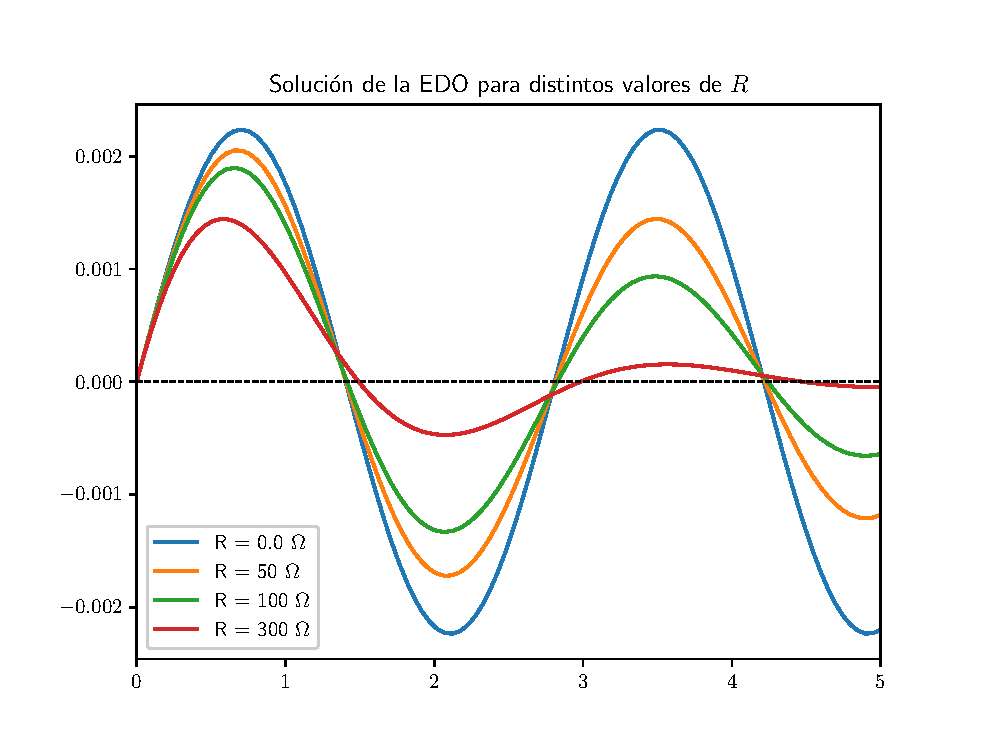
\includegraphics[scale=0.55]{Imagenes/plot_Ejercicio_odeint_03_Circuito_RLC.eps}
\end{figure}
\end{frame}
% \subsection{Sistema de 3 masas acopladas}
% \begin{frame}[fragile]
% \frametitle{Ejercicio 4 - Masas acopladas}
% En la figura se muestra un sistema de tres masas acopladas mediante resortes y amortiguadores.
% \begin{figure}
%     \centering
%     \includestandalone[scale=0.75]{Figuras/fig_edo_sist_3_masas}
% \end{figure}
% \end{frame}
% \begin{frame}[fragile]
% \frametitle{Ejercicio 4 - Masas acopladas}
% Los desplazamientos de estas tres masas satisfacen las ecuaciones dadas por:
% \fontsize{12}{12}\selectfont
% \begin{align*} 
%     M_{1} \: y^{\prime \prime}{1} + B_{1} \: y^{\prime}_{1} + K_{1} \: y_{1} - B_{1} \: y^{\prime}_{2} - K_{2} \: y_{2} & = F_{1}(t) \\
%     -B_{1} \: y^{\prime}_{1} - K_{1} \: y_{1} + M_{2} \:  y^{\prime \prime}_{2} + B_{1} \: y^{\prime}_{2} + (K_{1} + K_{2}) \: y_{2} - K_{2} \: y_{3} & = 0 \\
%     - K_{2} \: y_{2} + M_{3} \: y^{\prime \prime}_{3} + B_{2} \: y^{\prime}_{3} + (K_{2} + K_{3})  \: y_{3} & =  F_{3}(t) 
% \end{align*}
% \begin{figure}
%     \centering
%     \includestandalone[scale=0.75]{Figuras/fig_edo_sist_3_masas}
% \end{figure}
% \end{frame}
% \begin{frame}
% \frametitle{Condiciones iniciales}
% Las constantes y condiciones iniciales son
% \fontsize{12}{12}\selectfont
% \begin{tabbing}
% $K_{1} = K_{2} = K_{3} = 1$ \hspace{1.2cm} \= (constantes de los resortes, kgm/$s^{2}$) \\
% $M_{1} = M_{2} = M_{3} = 1$ \> (masa, kg) \\
% $F_{1}(t) = 1, F_{3}(t) = 0$ \> (fuerza, N) \\
% $B_{1} = B_{2} =0.1$ \> (coeficientes de amortiguamiento, kg/s) \\
% \\
% $y_{1}(0) = y^{\prime}_{1}(0) = y_{2}(0) = y^{\prime}_{2}(0) = y_{3}(0) = y^{\prime}_{3}(0) = 0$ \\
% \> (condiciones iniciales)
% \end{tabbing}
% \end{frame}
% \begin{frame}
% \frametitle{Problema a resolver}
% Resuelve el sistema para determinar la posición $y_{i}$ de cada masa en $0 \leq t \leq 60$ segundos, elabora una gráfica con las tres trayectorias.
% \end{frame}
% \begin{frame}
% \frametitle{Antes de proponer un código}
% Necesitamos manejar el sistema de 3 EDO2, de tal manera que podamos representar un sistema de 6 EDO1, entonces consideremos el siguiente:
% \\
% \bigskip
% Hint: Definiendo
% \[ y_{4} = y^{\prime}_{1}, \hspace{1cm} y_{5} = y^{\prime}_{2}, \hspace{1cm} y_{6} = y^{\prime}_{3} \]
% \end{frame}
% \begin{frame}
% \frametitle{Antes de proponer un código}
% Así, la ecuación inicial se escribe como un conjunto de seis EDO de primer orden, de la siguiente manera:
% \fontsize{12}{12}\selectfont
% \begin{align*}
% y^{\prime}_{1} & = y_{4} \\
% y^{\prime}_{2} & = y_{5} \\
% y^{\prime}_{3} & = y_{6} \\
% y^{\prime}_{4} & = \left[ -B_{1} \: y_{4} - K_{1} \: y_{1} + B_{1} \: y_{5} + K_{2} \: y_{2} + F_{1} \right] / M_{1} \\
% y^{\prime}_{5} & = \left[ B_{1} \: y_{4} + K_{1} \: y_{1} - B_{1} \: y_{5} - \left( K_{1} + K_{2} \right) \: y_{2} + K_{2} \: y_{3} \right] / M_{2}\\
% y^{\prime}_{6} & = \left[ K_{2} \: y_{2} - B_{2} \: y_{6} - \left( K_{2} + K_{3} \right) \: y_{3} + F_{3} \right] / M_{3}
% \end{align*}
% \end{frame}
% \begin{frame}[fragile, allowframebreaks, plain]
% \begin{lstlisting}[caption=Código para el sistema de masas, style=FormattedNumber, basicstyle=\linespread{1.1}\ttfamily=\small, columns=fullflexible]
% def F(y, t) : 
%     F = zeros(6)
%     F[_0_] = y[_3_]
%     F[_1_] = y[_4_]
%     F[_2_] = y[_5_]
%     F[_3_] = (-0.1 * y[_3_]- y[_0_] + 0.1 * y[_4_] + y[_1_] + 1.)
%     F[_4_] = (0.1 * y[_3_] + y[_0_] - 0.1 * y[_4_] - 2. * y[_1_] + y[_2_])
%     F[_5_] = (y[_1_] - 0.1 * y[_5_] - 2. * y[_2_])
%     return F

% t = linspace(0, 61, 100)
% y_0_ = array([0., 0., 0., 0., 0., 0.])

% sol = odeint(F, y_0_, t)

% plt.plot(t, sol[:,_0_], label = "$M{_1_}$")
% plt.plot(t, sol[:,_1_], label = "$M{_2_}$")
% plt.plot(t, sol[:,_2_], label = "$M{_3_}$")
% plt.legend(loc='upper right')
% plt.xlabel("Tiempo [s]")
% plt.ylabel("Amplitud")
% plt.axis([0, 60, -0.5, 6])
% plt.axhline(y=0, lw=0.75, ls='dashed', color='k')
% plt.title("Sistema de tres masas")
% plt.show()
% \end{lstlisting}
% \end{frame}
% \begin{frame}[plain]
% \frametitle{Solución al problema}
% \begin{figure}
%     \centering
%     \includegraphics[scale=0.65]{SistemaTresMasasRK4.eps} 
% \end{figure}
% \end{frame}
% \subsection{Sistema Lotka-Volterra}
% \begin{frame}
% \frametitle{Sistema Lotka-Volterra}
% Las ecuaciones de Lotka-Volterra, también son conocidas como ecuaciones de depredador-presa.
% \\
% \bigskip
% Está descrito por un sistema de 2 ecuaciones diferenciales no lineales de primer orden.
% \end{frame}
% \begin{frame}
% \frametitle{Sistema Lotka-Volterra}
% Se utiliza frecuentemente para describir la dinámica de sistemas biológicos donde interaccionan dos especies: un depredador y una de sus presas.
% \end{frame}
% \begin{frame}
% \frametitle{Sistema de ecuaciones acopladas}
% El sistema evoluciona de acuerdo al par de ecuaciones:
% \begin{align*}
% \dfrac{du}{dt} &= a \: u - b \: u \: v \\
% \dfrac{dv}{dt} &= -c \: v + d \: b\: u\: v
% \end{align*}
% donde:  
% \setbeamercolor{item projected}{bg=yellow!80!black,fg=black}
% \setbeamertemplate{enumerate items}[circle]
% \begin{enumerate}[<+->]
% \item $u$ es el número de presas (ej. Conejos)
% \item $v$ es el número de depredadores (ej. Zorros)
% \seti
% \end{enumerate}
% \end{frame}
% \begin{frame}
% \frametitle{Sistema de ecuaciones acopladas}
% \begin{align*}
% \dfrac{du}{dt} &= a \: u - b \: u \: v \\
% \dfrac{dv}{dt} &= -c \: v + d \: b\: u\: v
% \end{align*}
% donde:
% \setbeamercolor{item projected}{bg=yellow!80!black,fg=black}
% \setbeamertemplate{enumerate items}[circle]
% \begin{enumerate}[<+->]
% \conti
% \item $a$ es la tasa natural de crecimiento de conejos, sin que haya zorros.
% \item $b$ es la tasa natural de la muerte de conejos, debido a la depredación.
% \seti
% \end{enumerate}
% \end{frame}
% \begin{frame}
% \frametitle{Sistema de ecuaciones acopladas}
% \begin{align*}
% \dfrac{du}{dt} &= a \: u - b \: u \: v \\
% \dfrac{dv}{dt} &= -c \: v + d \: b\: u\: v
% \end{align*}
% donde:
% \setbeamercolor{item projected}{bg=yellow!80!black,fg=black}
% \setbeamertemplate{enumerate items}[circle]
% \begin{enumerate}[<+->]
% \conti
% \item $c$ es la tasa natural de la muerte del zorro, cuando no hay conejos.
% \item $d$ es el factor que describe el número de conejos capturados.
% \end{enumerate}
% \end{frame}
% \begin{frame}
% \frametitle{Poblaciones iniciales}
% Vamos a utilizar $X = [u, v]$ para describir el estado de las poblaciones.
% \end{frame}
% \begin{frame}[plain, fragile]
% \frametitle{Definiendo las ecuaciones}
% \begin{lstlisting}[caption=Código inicial, style=FormattedNumber, basicstyle=\linespread{1.1}\ttfamily=\small, columns=fullflexible]
% from numpy import *
% import matplotlib.pyplot as plt

% a = 1.
% b = 0.1
% c = 1.5
% d = 0.75

% def dXdt(X, t = 0):
%     return array([ a * X[_0_] - b * X[_0_] * X[_1_], -c * X[_1_] + d * b * X[_0_] * X[_1_] ])
% \end{lstlisting}
% \end{frame}
% \begin{frame}[plain, fragile]
% \frametitle{Población en equilibrio}
% Antes de usar \funcionazul{odeint} para integrar el sistema, veremos de cerca la posición de equilibrio.
% \\
% \bigskip
% El equilibrio ocurre cuando la tasa de crecimiento es igual a $0$, lo que nos da dos puntos fijos:
% \begin{lstlisting}[caption=Equilibrio en las poblaciones, style=FormattedNumber, basicstyle=\linespread{1.1}\ttfamily=\small, columns=fullflexible]
% Xf_0_ = array([0., 0.])
% Xf_1_ = array([ c/(d * b), a/b])
% all(dXdt(Xf_0_) == zeros(_2_) ) and all(dXdt(Xf1) == zeros(_2_))
% \end{lstlisting}
% \end{frame}
% \begin{frame}[fragile]
% \frametitle{Variable temporal y cond. iniciales}
% Para usar la función \funcionazul{odeint}, hay que definir el parámetro de tiempo $t$, así como las condiciones inciales de la población: $10$ conejos y $5$ zorros.
% \end{frame}
% \begin{frame}[fragile]
% \frametitle{Variable temporal y cond. iniciales}
% \begin{lstlisting}[caption=Código para las condiciones iniciales, style=FormattedNumber, basicstyle=\linespread{1.1}\ttfamily=\small, columns=fullflexible]
% t = linspace(0, 15,  1000)
              
% X_0_ = array([10, 5])         
            
% X = integrate.odeint(dXdt, X_0_, t)
% \end{lstlisting}
% \end{frame}
% \begin{frame}
% \frametitle{Graficando la solución}
% Una vez obtenido el código para la solución del problema, ahora nos corresponde graficar el conjunto de datos obtenido:
% \end{frame}
% \begin{frame}[fragile, plain, allowframebreaks]
% \frametitle{Graficando la solución}
% \begin{lstlisting}[caption=Código para graficar, style=FormattedNumber, basicstyle=\linespread{1.1}\ttfamily=\small, columns=fullflexible]
% conejos, zorros = X.T

% f_1_ = plt.figure()
% plt.plot(t, conejos, 'r-', label='Conejos')
% plt.plot(t, zorros  , 'b-', label='Zorros')
% plt.grid()
% plt.legend(loc='best')
% plt.xlabel('tiempo')
% plt.ylabel('poblacion')
% plt.title('Evolucion de la poblacion de conejos y zorros')
% plt.show()
% \end{lstlisting}
% \end{frame}
% \begin{frame}[plain]
% \frametitle{Resultado gráfico}
% \begin{figure}
%     \centering
%     \includegraphics[scale=0.6]{Imagenes/LotkaVolterra_01.eps} 
% \end{figure}
% \end{frame}
% \begin{frame}
% \frametitle{Primer resultado}
% La gráfica anterior nos da la información sobre el número tanto de conejos como de zorros durante el intervalo de tiempo estudiado, es decir, tenemos una especie de \enquote{censo}.
% \\
% \medskip
% Para ver la dinámica de las poblaciones propiamente, ahora representamos el espacio fase del sistema, por lo que tenemos que hacer algunos ajustes en el código que usamos anteriormente.
% \end{frame}
% \begin{frame}[fragile]
% \frametitle{Condiciones de equilibrio}
% Consideremos las condiciones de equilibrio, es decir, donde la tasa de crecimiento es cero:
% \begin{lstlisting}[caption=Condiciones de equilibrio, style=FormattedNumber, basicstyle=\linespread{1.1}\ttfamily=\small, columns=fullflexible]
% Xf_0_ = array([0. , 0.])
% Xf_1_ = array([ c/(d * b), a/b])
% \end{lstlisting}
% \end{frame}
% \begin{frame}[fragile]
% \frametitle{Elementos adicionales para la gráfica}
% Dibujaremos el espacio fase con algunos elementos visuales con el fin de decoración nada más.
% \begin{lstlisting}[caption=Obteniendo los colores, style=FormattedNumber, basicstyle=\linespread{1.1}\ttfamily=\small, columns=fullflexible]
% values  = linspace(0.3, 0.9, 5)                         

% vcolors = plt.cm.autumn_r(linspace(0.3, 1., len(values)))  

% f2 = plt.figure()
% \end{lstlisting}
% \end{frame}
% \begin{frame}[fragile]
% \frametitle{El módulo \texttt{color map}}
% El módulo \funcionazul{cm} proporciona un conjunto de mapas de colores predeterminados, así como las funciones necesarias para crear nuevos mapas de color.
% \end{frame}
% \begin{frame}[fragile]
% \frametitle{El módulo \texttt{color map}}
% Existen varios mapas ya definidos: \funcionazul{autumn, bone, cool, copper, flag, gray, hot, hsv, jet, pink, prism, spring, summer, winter, spectral}.
% \end{frame}
% \begin{frame}[plain, fragile]
% \frametitle{Curvas de nivel}
% Se van a dibujar ahora las trayectorias para diferentes condiciones iniciales (número de conejos y zorros)
% \begin{lstlisting}[caption=Graficando las curvas de nivel, style=FormattedNumber, basicstyle=\linespread{1.1}\ttfamily=\small, columns=fullflexible]
% for v, col in zip(values, vcolors):
%     X_0_ = v * Xf_1_
    
%     X = integrate.odeint( dXdt, X_0_, t)

%     plt.plot( X[:,_0_], X[:,_1_], lw=3.5 * v, color=col, label='X_0_=(%.f, %.f)' % ( X_0_[_0_], X_0_[_1_]) )
% \end{lstlisting}
% \end{frame}
% \begin{frame}[fragile]
% \frametitle{La función \texttt{zip}}
% La función \funcionazul{zip} sirve para reorganizar las listas en \python.
% \\
% \bigskip
% Como parámetros admite un conjunto de listas. 
% \end{frame}
% \begin{frame}[fragile]
% \frametitle{La función \texttt{zip}}
% Lo que realmente hace es tomar el elemento i-ésimo elemento de cada lista y los une en una tupla, después une todas las tuplas en una lista.
% \\
% \medskip
% En cada gráfica se modificará el grosor de la línea y el color que se le asocia.
% \end{frame}
% \begin{frame}[fragile]
% \frametitle{Definición de una malla}
% Se define una malla sobre nuestro espacio de solución:
% \begin{lstlisting}[caption=Creando una malla, style=FormattedNumber, basicstyle=\linespread{1.1}\ttfamily=\small, columns=fullflexible]
% ymax = plt.ylim(ymin = 0)[_1_]
% xmax = plt.xlim(xmin = 0)[_1_]

% nbpoints   = 20

% x = linspace(0, xmax, nbpoints)
% y = linspace(0, ymax, nbpoints)

% X_1_, Y_1_  = meshgrid(x, y)
% \end{lstlisting}
% \end{frame}
% \begin{frame}
% \frametitle{¿Qué hace \texttt{meshgrid}?}
% La función \funcionazul{meshgrid} genera un arreglo n-dimensional para evaluaciones vectoriales de campos n-dimensionales ya sea escalares o vectoriales, a partir de arreglos unidimensionales $x_{1}, x_{2}, \ldots, x_{n}$.
% \end{frame}
% \begin{frame}[fragile]
% \frametitle{Calculando la magnitud del vector}
% \begin{lstlisting}[caption=Magnitud del vector y su dirección, style=FormattedNumber, basicstyle=\linespread{1.1}\ttfamily=\small, columns=fullflexible]
% DX_1_, DY_1_ = dXdt([X_1_, Y_1_])                      

% M = (hypot(DX_1_, DY_1_))                           

% M[ M == 0] = 1.                                 

% DX_1_ /= M                                        
% DY_1_ /= M
% \end{lstlisting}
% \end{frame}
% \begin{frame}[fragile]
% \frametitle{Calculando la magnitud del vector}
% \setbeamercolor{item projected}{bg=yellow!80!black,fg=black}
% \setbeamertemplate{enumerate items}[circle]
% \begin{enumerate}[<+->]
% \item Con \texttt{X1} y \texttt{Y1} se crea una malla. 
% \item Con \texttt{DX1} y \texttt{DY1} se calcula el crecimiento de las poblaciones en la malla.
% \item Con la variable \texttt{M} se calcula la norma de la tasa de crecimiento, usando la función \funcionazul{hypot}.
% \item La expresión \texttt{M[M==0] =1.} evita que tengamos una división entre cero.
% \item Con la operación \texttt{DX1/M} y \texttt{DY1/M} se normaliza cada vector.
% \end{enumerate}
% \end{frame}
% \begin{frame}[plain, allowframebreaks, fragile]
% \frametitle{Dibujando las direcciones del vector}
% Se dibujan las direcciones usando \funcionazul{quiver}
% \begin{lstlisting}[caption=Dibujando las direcciones del vector resultante, style=FormattedNumber, basicstyle=\linespread{1.1}\ttfamily=\small, columns=fullflexible]
% plt.title('Trayectorias y campo de direccion')

% Q = plt.quiver(X_1_, Y_1_, DX_1_, DY_1_, M, pivot='mid', cmap=plt.cm.jet)

% plt.xlabel('Numero de conejos')
% plt.ylabel('Numero de zorros')
% plt.legend()
% plt.grid()
% plt.xlim(0, xmax)
% plt.ylim(0, ymax)
% plt.show()
% \end{lstlisting}
% \end{frame}
% \begin{frame}[fragile]
% \frametitle{La función \texttt{quiver}} 
% La función \funcionazul{quiver} genera el mapa vectorial, requiere de cinco argumentos: las posiciones $X1$,$Y1$ de inicio, el valor de las componentes del vector $DX1$, $DY1$ y el color asociado, el argumento \texttt{pivot} indica en qué parte de la malla se va a colocar el vector.
% \end{frame}
% \begin{frame}[plain]
% \frametitle{Resultado gráfico}
% \begin{figure}
%     \centering
%     \includegraphics[scale=0.5]{LotkaVolterra_02.eps} 
% \end{figure}
% \end{frame}
% \begin{frame}
% \frametitle{Ejercicio para resolver}
% El modelo de Lorenz se usa para estudiar la formación de torbellinos en la atmósfera, aunque abordó el problema de manera general, estableció las bases para el estudio de sistemas dinámicos.
% \end{frame}
% \begin{frame}
% \frametitle{Ejercicio para resolver}
% El conjunto de ecuaciones está dado por
% \begin{align*}
% \dfrac{dy_{1}}{dt} &= a(y_{2} - y_{1}) \\
% \dfrac{dy_{2}}{dt} &= (b - y_{3}) \: y_{1} - y_{2} \\
% \dfrac{dy_{3}}{dt} &= y_{1} \: y_{2} - c \: y_{3}
% \end{align*}
% en el modelo $a$, $b$ y $c$ son parámetros positivos. 
% \end{frame}
% \begin{frame}
% \frametitle{Ejercicio para resolver}
% Resuelve este modelo numéricamente y grafica la solución.
% \\
% \bigskip
% Utiliza los siguientes valores $a = 10$, $b = 28$ y $c =    8/3$. Interpreta la solución.
% \end{frame}
% \begin{frame}[plain]
% \frametitle{Resultado gráfico}
% \begin{figure}
%     \centering
%     \includegraphics[scale=0.5]{Lorenz_01.eps} 
% \end{figure}
% \end{frame}
% \begin{frame}[fragile]
% \frametitle{Para generar una gráfica 3D}
% Para graficar una función de tres variables en \funcionazul{matplotlib}, debemos de utilizar una combinación de dos librerías:
% \begin{verbatim}
% import matplotlib.pyplot as plt
% import mpl_toolkits.mplot3d.axes3d as p3
% \end{verbatim}    
% \end{frame}
% \begin{frame}[fragile]
% \frametitle{Usando \texttt{plot3D}}
% Hay un importante cambio cuando graficamos tres variables con \funcionazul{matplotlib}, hay adecuar el espacio de trabajo mediante la siguiente referencia:
% \begin{verbatim}
% fig = plt.figure()

% ax = p3.Axes3D(fig)
% \end{verbatim}
% Con \texttt{plt} definimos el espacio común de graficación, pero con \texttt{ax}, ahora y contamos con la manera de usar la graficación de tres variables.
% \end{frame}
% \begin{frame}[fragile]
% \frametitle{La función \texttt{plot3D}}
% La función \funcionazul{plot3D} ocupa los argumentos de la misma manera que \funcionazul{plot}, por lo que debemos de usar la sintaxis:
% \begin{verbatim}
% ax.plot3D(x, y, z)

% ax.set_xlabel('X')
% ax.set_ylabel('Y')
% ax.set_zlabel('Z')

% fig.add_axes(ax)
% plt.show()
% \end{verbatim}
% \end{frame}

\end{document}
